%%%%%%%%%%%%%%%%%%%%%%%%%%%%%%%%%%%%%%%%%%%%%%%%%%%%%%%%%%%%%%%%%%%%%%%%%%%%%%%%
%2345678901234567890123456789012345678901234567890123456789012345678901234567890
%        1         2         3         4         5         6         7         8

%\documentclass[12pt, draftcls, onecolumn]{IEEEtran}
\documentclass[journal]{IEEEtran}

 
\IEEEoverridecommandlockouts                              % This command is only
                                                          % needed if you want to
                                                          % use the \thanks command

\usepackage{amsmath}    % need for sub equations
\usepackage{amsfonts}
\usepackage{graphicx}   % need for figures
\usepackage{subcaption}
\usepackage{epsfig} 
\usepackage{algorithmic}
\usepackage{color}
\usepackage[normalem]{ulem}
\usepackage{cancel}
\usepackage{amssymb}
\usepackage{color}

\usepackage[ruled,vlined,titlenotnumbered]{algorithm2e} 
\usepackage{cite}
\usepackage{float}

\newcommand{\R}{\mathbb{R}}
\newcommand{\xset}{\mathcal{X}}
\newcommand{\yset}{\mathcal{Y}}
\newcommand{\xfset}{\mathbb{X}}
\newcommand{\yfset}{\mathbb{Y}}

\newcommand{\reachset}{\mathcal{V}}
\newcommand{\targetset}{\mathcal{L}}
\newcommand{\traj}{\zeta} % trajectory


\newcommand{\pcset}{\mathcal{U}_p} %planner control set
\newcommand{\pcfset}{\mathbb{U}_p} %planner control function set
\newcommand{\tcset}{\mathcal{U}_s} %tracker control set
\newcommand{\tcfset}{\mathbb{U}_s} %tracker control funciton set
\newcommand{\dset}{\mathcal{D}}
\newcommand{\dfset}{\mathbb{D}}

\newcommand{\pset}{\mathcal{P}} %planner set set
\newcommand{\tset}{\mathcal{S}} %tracker set
\newcommand{\rset}{\mathcal{R}}

\newcommand{\tvar}{t}
\newcommand{\thor}{T} % Time horizon

\newcommand{\tstate}{s} % Tracker state
\newcommand{\pstate}{p} % Planner state
\newcommand{\rstate}{r} % Relative state


\newcommand{\ttraj}{\xi_{\tdyn}} % Tracker trajectory
\newcommand{\ptraj}{\xi_{\pdyn}} %Planner trajectory
\newcommand{\rtraj}{\xi_\rdyn}

\newcommand{\senseDist}{m}


\newcommand{\tctrl}{u_s} % Tracker control
\newcommand{\dstb}{d} % Disturbance
\newcommand{\pctrl}{u_p} % Planner control

\newcommand{\tdyn}{f} % Tracker dynamics
\newcommand{\pdyn}{h} % Planner Dynamics
\newcommand{\rdyn}{g} % Relative dynamics

\newcommand{\plannerfunc}{j}

\newcommand{\ptind}{i} % Index of vehicle state corresponding to planner state
\newcommand{\ptmat}{Q} % Matrix for transforming planner state to the same length as tracker state
\newcommand{\tpmat}{Q^T}

\newcommand{\errfunc}{l} % Error function
\newcommand{\valfunc}{V} % Value function
\newcommand{\walfunc}{W} % Value function

\newcommand{\deriv}{\nabla\valfunc} %gradient look-up table

\newcommand{\dx}{\Delta x} %distance allowed in a time step
\newcommand{\dt}{\Delta t} %time step

\newcommand{\obsSense}{\mathcal{O}_{sense}}
\newcommand{\obsAug}{\mathcal{O}_{aug}}



\newcommand{\TEB}{\mathcal B} % tracking error bound

\newtheorem{thm}{Theorem}
\newtheorem{claim}{Claim}
\newtheorem{rem}{Remark}
\newtheorem{prop}{Proposition}
\newtheorem{proof}{IEEEproof}

\newcommand{\MCnote}{\textcolor{blue}}
\newcommand{\SHnote}{\textcolor{red}}

\title{\LARGE \bf FaSTrack Journal Version}

\author{}
%\author{Sylvia L. Herbert*, Mo Chen*, SooJean Han, Somil Bansal, Jaime F. Fisac, and Claire J. Tomlin
%\thanks{This research is supported by ONR under the Embedded Humans MURI (N00014-16-1-2206). The research of S. Herbert has received funding from the NSF GRFP and the UC Berkeley Chancellor's Fellowship Program.}
%\thanks{* Both authors contributed equally to this work. All authors are with the Department of Electrical Engineering and Computer Sciences, University of California, Berkeley. \{sylvia.herbert, mochen72, soojean, somil, jfisac, tomlin\}@berkeley.edu}}


\begin{document}
\maketitle
\thispagestyle{empty}
\pagestyle{empty}

%%%
\begin{abstract}
Real-time and safe trajectory planning in unknown environments is vital to many applications of autonomous systems. Real-time trajectory planning typically requires simplified system dynamics planning at best, while safe trajectory planning tends to be computationally intensive. We propose FaSTrack, Fast and Safe Tracking, . A path or trajectory planner using simplified dynamics to plan quickly can be incorporated into the FaSTrack framework, which provides a safety controller for the vehicle along with a guaranteed tracking error bound. This bound captures all possible deviations due to high dimensional dynamics and external disturbances. Note that FaSTrack is modular and can be used with most current path or trajectory planners. We demonstrate this framework using a 10D nonlinear quadrotor model tracking a 3D path obtained from an RRT planner.
\end{abstract}

% !TEX root = tracking.tex
\section{Introduction}
 As unmanned aerial vehicles (UAVs) and other autonomous systems become more commonplace, it is essential that they be able to plan safe motion paths through crowded environments in real-time. This is particularly crucial for navigating through environments that are \textit{a priori} unknown, because re-planning based on updated information about the environment is often necessary. 
 However, for many common dynamical systems, accurate and robust path planning can be too computationally expensive to perform efficiently. 
 In order to achieve real-time planning, many algorithms use highly simplified model dynamics or kinematics, resulting in a tracking error between the planned path and the true high-dimensional system. 
 This concept is illustrated in Fig. \ref{fig:chasing}, where the path was planned using a simplified planning model, but the real vehicle cannot track this path exactly. 
 In addition, external disturbances (e.g. wind) can be difficult to account for. Crucially, such tracking errors can lead to dangerous situations in which the planned path is safe, but the actual system trajectory enters unsafe regions.
 
 %Real-time planning that is both safe and accurate presents a very difficult challenge: accuracy and robustness in many dyanimcal systme sis difficult to compute, often precluding real-time computer hands.fast planning is generally at odds with the need for maintaining safety and robustness.  

We propose the modular tool FaSTrack: Fast and Safe Tracking, which models the navigation task as a sophisticated \textit{tracking system} that pursues a simplified \textit{planning system}. 
The tracking system accounts for complex system dynamics as well as bounded external disturbances, while the simple planning system enables the use of real-time planning algorithms. 
Offline, a precomputed pursuit-evasion game between the two systems can be analyzed using any suitable method. 
This results in a \textit{tracking error function} that maps the initial relative state between the two systems to the \textit{tracking error bound} (TEB): the maximum possible relative distance that could occur over time. 
This TEB can be thought of as a ``safety bubble" around the planning system that the tracking system is guaranteed to stay within. 
Because the tracking error is bounded in the relative state space, we can precompute and store a \textit{safety control function} that  maps the real-time relative state to the optimal safety control for the tracking system to ``catch" the planning system. 
The offline computations are \textit{independent} of the path planned in real-time.

Online, the autonomous system senses obstacles, which are then augmented by the TEB to ensure that no potentially unsafe paths can be computed. 
Next, a path or trajectory planner uses the simplified planning model to determine the next desired state. 
The tracking system then finds the relative state between itself and the next desired state. 
If this relative state is nearing the TEB then it is plugged into the safety control function to find the instantaneous optimal safety control of the tracking system; otherwise, any controller may be used. In this sense, FaSTrack provides a \emph{least-restrictive} control law. 
This process is repeated as long as desired. 
  
\begin{figure}
	\centering
	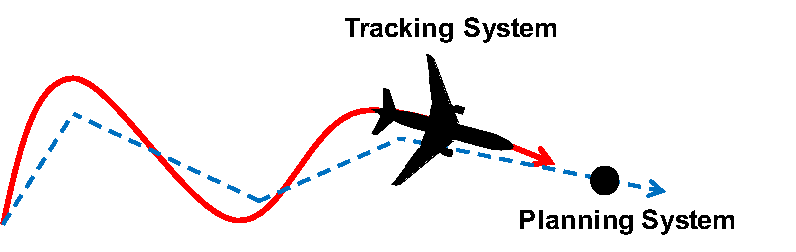
\includegraphics[width=0.35\textwidth]{fig/chasing}
	\caption{Left: A planning system (blue disk) using a fast but simple model, followed by a tracking system (green plane) using a more complex model, navigating through an environment with obstacles; the tracking system is guaranteed to stay within some TEB (blue circle). Right: Safety and goal-satisfaction can be guaranteed by planning with respect to augmented obstacles (large blue circles).}
	\label{fig:chasing}
\end{figure}
%

FaSTrack to be modular, and it can be used with any method for computing the TEB in conjunction with any existing fast path or trajectory planners, enabling motion planning that is real-time, guaranteed safe, and dynamically accurate. 
In this paper, we demonstrate this tool by computing the TEBs solving a Hamilton-Jacobi (HJ) partial differential equation (PDE), and using a different planning algorithm for each numerical example. 
In the three examples, we also consider different models for the tracking system and the planning system.
In the simulations, the system travels through a static environment with constraints defined, for example, by obstacles, while experiencing disturbances.
The constraints are only fully known through online sensing, for example, once obstacles are within the limited sensing region of the vehicle. 
Combining this TEB with real-time planners the system is able to safely plan and track a trajectory through the environment in real time. 
The planning algorithms used in our numerical examples are the fast sweeping method (FSM) \cite{Takei2013}, rapidly-exploring random trees (RRT) \cite{Kuffner2000,Kavraki1996}, and model-predictive control (MPC) \cite{Qin2003}.
% Introduction (.5-1p)
%%Tracking with quadrotors is a need
%%There exist methods that work in real time and methods that work for safety but not very many for both
%%Goal: combine both in a simple way

% !TEX root = tracking.tex
\section{Related Work \label{sec:relatedwork}}
Motion planning is a very active area of research in the controls and robotics communities \cite{Hoy2015}.  In this section we will discuss past work on path planning, kinematic planning, and dynamic planning.  A major current challenge is to find an intersection of robust, nonlinear, and real-time planning. 

There is a wealth of research in the area of sample-based path planning.  Planning methods like rapidly-exploring random trees (RRT) \cite{Kuffner2000}, probabilistic road maps (PRM) \cite{Kavraki1996}, and fast marching tree (FMT) \cite{Janson2015} can find collision-free paths through known or partially known environments.  These paths can then be smoothed with shortcut-based methods or turned into optimal motion plans \cite{Richter2016, Karaman2011, Kobilarov2012}.  These systems work well in many applications, but are not designed to be robust to model uncertainty or disturbances.

Motion planning for kinematic systems can also be accomplished through online trajectory optimization using methods such as TrajOpt \cite{Schulman2013} and CHOMP \cite{Ratliff2009}. These methods can work extremely well in many applications, but are generally challenging to implement for real-time nonlinear dynamic systems due to the computational load.

Model predictive control (MPC) has been a very successful method for dynamic trajectory optimization in both academia and industry \cite{Qin2003}.  However, combining speed, safety, and complex dynamics is a difficult balance to achieve. Using MPC for robotic and aircraft systems typically requires reducing the system complexity to take advantage of linear programming or mixed integer linear programming (MILP) \cite{Alexis2016, Bellingham2002, Vitus2008, Zeilinger2011, Richter2012}. Robustness in linear systems can be achieved using constraint tightening MPC to balance speed with safety \cite{Kuwata2007, Richards2006} or reference tracking \cite{DiCairano2016}. Nonlinear MPC is most often used on systems that evolve more slowly over time \cite{Diehl2002, Schildbach2016}, but there is active work to speed computation using Newton type methods and structure exploitation \cite{Diehl2009, Quirynen2015, Grune2011, Neunert2016}. Adding robustness to nonlinear MPC is being explored through algorithms based on minimax formulation and tube MPCs that bound output trajectories of a system with a tube around a nominal path (see survey paper \cite{Hoy2015} for references).
%speed nonlinear: Findeisen2007,Gupta2015, Torrisi2016

%learning through neural networks \cite{Yan2014}, 
%minimax \cite{Lofberg2003, Kumar2014}
% tube \cite{Mayne2011, Cannon2011, Kumar2014, Gao2014}

There are other methods of dynamic trajectory planning that manage to cleverly skirt the issue of solving for optimal trajectories online.  One such method works by storing a fixed precomputed set of trajectories called motion primitives that are then selected and composed together online.  This has been remarkably useful in many practical applications \cite{Gillula2010, Dey2016, Barry2016}, and there is impressive work on making these systems robust using funnels \cite{Majumdar2016}.  Another tactic for online dynamic trajectory planning involves the generation of several random trajectories at each waypoint, and then picking the best of those computed \cite{Kalakrishnan2011, Schwesinger2013, Krusi2015}.  This method works well in many applications, but is risky in its reliance on finding randomly-generated collision-free trajectories. 

There are also motion planning methods that are designed to be robust. Control barrier functions \cite{Xu2015, Ames2014} place inequality constraints in the control input that allow for dynamic trajectory planning as a quadratic program. New work in planning using contraction theory works by forming safe tubes online around a nominal dynamic trajectory \cite{Singh2017}.

Offline planners like Hamilton-Jacobi reachability analysis can find control policies and guarantees for nonlinear systems that avoid obstacles and are robust to bounded disturbances \cite{Mitchell05}.  However, this method can only approach real-time speed for very low-dimensional (1D-2D) systems. Although there has been work to speed up analysis by decomposing high-dimensional systems into smaller subsystems \cite{Chen2016a, Chen2016b}, dimensionality is still a common hurdle.

The work presented in this paper differs from the robust planning methods above because it is designed to be modular and easy to use in conjunction with a number of path and trajectory planners. Additionally, FASTrack can handle bounded external disturbances (e.g. wind) and work with both known and unknown environments with static obstacles. 
% Related Work (1p)
%%work on fast planning
%%work on safe planning
%%work on both
%%how ours is different

% !TEX root = tracking.tex
\section{Problem Formulation \label{sec:formulation}}
We seek to simultaneously plan and track a trajectory (or path converted to a trajectory) online in real time. Planning is done using a kinematic or dynamic planning model. Tracking is done by a tracking model representing the autonomous system. The environment may contain static obstacles that are either known a priori or can be observed by the system within a limited sensing range (see Section \ref{sec:online}).

\subsection{Tracking Model}
The tracking model represents the autonomous system dynamics, and in general may be nonlinear and high-dimensional. Let $\tstate$ represent the state variables of the tracking model, which evolves according to
\begin{equation}
\begin{aligned}
\label{eq:tdyn}
\dot{\tstate} = \tdyn(\tstate, \tctrl, \dstb), \tvar \in [0, \thor], \tstate \in \tset, \tctrl \in \tcset, \dstb \in \dset.
\end{aligned}
\end{equation}
We assume that the system dynamics $\tdyn : \tset\ \times\ \tcset \times \dset \rightarrow \tset$ are uniformly continuous, bounded, and Lipschitz continuous in $\tstate$ for fixed control $\tctrl$. The control function $\tctrl(\cdot)$ and disturbance function $\dstb(\cdot)$ are drawn from the following sets:
\begin{equation}
\begin{aligned}
\tctrl(\cdot) \in \tcfset(t) = \{\phi: [0, \thor] \rightarrow \tcset: \phi(\cdot) \text{ is measurable}\},\\
\dstb(\cdot) \in \dfset(t) = \{\phi: [0, \thor] \rightarrow \dset: \phi(\cdot) \text{ is measurable}\},
\end{aligned}
\end{equation}
where $\tcset, \dset$ are compact and $t\in[0, \thor]$ for some $T>0$. Under these assumptions there exists a unique trajectory solving (\ref{eq:tdyn}) for a given $\tctrl(\cdot) \in \tcset$ \cite{Coddington84}. The trajectories of (\ref{eq:tdyn}) that solve this ODE will be denoted as $\ttraj(\tvar; \tstate, \tvar_0, \tctrl(\cdot))$, where $\tvar_0,\tvar \in [0, \thor]$ and $\tvar_0 \leq \tvar$. These trajectories satisfy
\begin{equation}
\label{eq:fdyn_traj}
\begin{aligned}
\dot\ttraj(\tvar; \tstate, \tvar_0, \tctrl(\cdot)) &= \tdyn(\ttraj(\tvar; \tstate, \tvar_0, \tctrl(\cdot)), \tctrl(\tvar)), \\
\ttraj(\tvar; \tstate, \tvar, \tctrl(\cdot)) &= \tstate.
\end{aligned}
\end{equation}

\subsection{Planning Model}
The planning model is used by the path or trajectory planner to determine a desired path online. Kinematics or low-dimensional dynamics are typically used depending on the requirements of the planner. Let $\pstate$ represent the state variables of the planning model, with control $\pctrl$. The planning states $\pstate \in \pset$ are a subset of the tracking states $\tstate \in \tset$. The dynamics similarly satisfy 
\begin{equation}
\begin{aligned}
\label{eq:pdyn}
\dot{\pstate} = \pdyn(\pstate, \pctrl), \tvar \in [0, \thor], \pstate \in \pset, \ \underline{\pctrl} \leq \pctrl \leq \overline{\pctrl}.
\end{aligned}
\end{equation}
Note that the planning model does not involve a disturbance input. This is a key feature of FaSTrack: the treatment of disturbances is only necessary in the tracking model, which is modular with respect to any planning method, including those that do not account for disturbances.

\subsection{Goals of This Paper}
The goals of the paper are threefold:
\begin{enumerate}
	\item To provide a tool for precomputing functions (or look-up tables) to determine a guaranteed tracking error bound between tracking and planning models, and optimal safety controller for robust motion planning with nonlinear dynamic systems
	\item To develop a framework for easily implementing this tool with fast real-time path and trajectory planners.
	\item To demonstrate the tool and framework in an example using a high dimensional system
\end{enumerate}

% formally introduce the problem

% !TEX root = tracking.tex
\section{General Framework \label{sec:framework}}
To achieve our goals, we propose FaSTrack, a framework that decouples the formal guarantee of safety from the planning algorithm.
Instead of having the system, represented by the tracking model, directly plan trajectories towards $\goal$, in our framework the tracking system ``chases'' the planning system, which uses any planning algorithm to obtain trajectories in real-time.
Safety is formally guaranteed through a precomputed of a TEB along with a corresponding tracking controller, in combination with augmentation of constraints based on this TEB.
An illustrate of our framework is shown in Figure \ref{fig:chasing}.

More details of the framework is summarized in Figs. \ref{fig:fw_online}, \ref{fig:hybrid_ctrl}, \ref{fig:fw_offline}. 
The online real-time framework is shown in Fig. \ref{fig:fw_online}. 
At the center of this framework is the path or trajectory planner; our framework is agnostic to the planner, so any may be used (e.g. MPC, RRT, neural networks). 
We will present three example using FSM, RRT, and MPC planners in Section \ref{sec:results}.
\begin{figure}[h!]
  \centering
	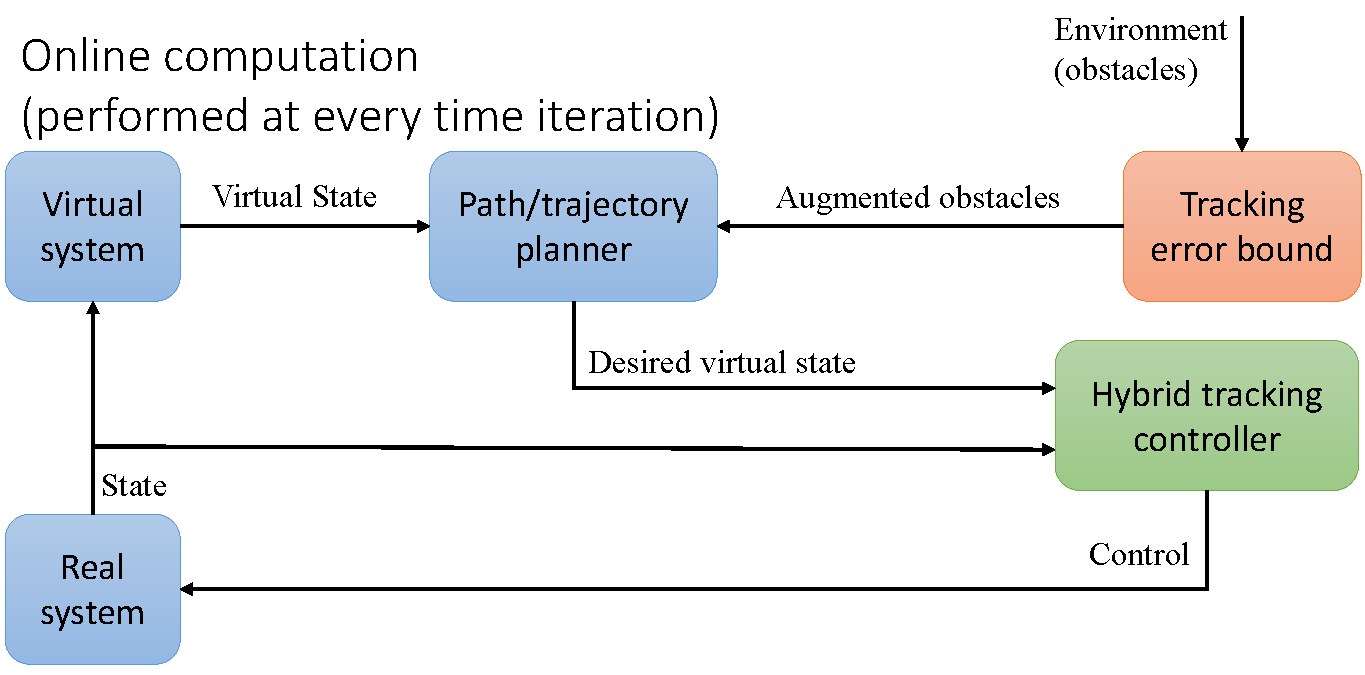
\includegraphics[width=1\columnwidth]{fig/framework_online}
	\caption{Online framework}
	\label{fig:fw_online}
	\vspace{-.1in}
\end{figure}

When executing the online framework, the first step is to sense obstacles in the environment, and then augment the sensed obstacles by a precomputed tracking error bound as described in Section \ref{sec:precomp}. This tracking error bound is a safety margin that guarantees robustness despite the worst-case disturbance. Augmenting the obstacles by this margin can be thought of as equivalent to wrapping the planning system with a ``safety bubble". These augmented obstacles are given as inputs to the planner along with the current state of the planning system. The planner then outputs the next desired state of the planning system. 

The tracking system is a model of the physical system (such as a quadrotor). The hybrid tracking controller block takes in the state of the tracking system as well as the desired state of the planning system. Based on the relative state between these two systems, the hybrid tracking controller outputs a control signal to the tracking system. The goal of this control is to make the tracking system track the desired planning state as closely as possible.

%In the context of real-time robust planning towards a target in an unknown environment, we propose a framework for combining fast planning methods that do not need to take into account disturbances, and HJ reachability analysis which provides formal guarantees for systems with disturbances. The high level idea of the framework is summarized in Fig. \ref{fig:fw_online}, \ref{fig:hybrid_ctrl}, and \ref{fig:fw_offline}. Formal definitions will be introduced in \MCnote{Section \ref{}}.

%Fig. \ref{fig:fw_online} shows the online computations under our framework, which uses a hierarchical structure in which a planner plans a path or trajectory for a simple ``virtual system''. Examples of planners include those based on model-predictive control (MPC), rapidly-exploring random tree (RRT), or neural networks; our framework is agnostic to the planner, so any planner can be used. The choice of the virtual system is also flexible, and depends on the requirements of the planner. We will present an example of a virtual system used in conjunction with an RRT planner in \MCnote{Section \ref{}}. The planner outputs a desired ``virtual state'' of the virtual system.

%The ``real system'' is a model of a physical system such as a quadrotor, and a subset of the state variables forms the virtual state of the virtual system. The state of real system and the desired virtual state are inputs to a hybrid tracking controller. Based on these two inputs, the hybrid tracking controller outputs a control signal to the real system. The goal of this control is to make the real system track the desired virtual state as closely as possible. Our concept of tracking error will be defined in \MCnote{Section \ref{}}.

The hybrid tracking controller is expanded in Fig. \ref{fig:hybrid_ctrl} and consists of two controllers: a safety controller and a performance controller. In general, there may be multiple safety and performance controllers depending on various factors such as observed size of disturbances, but for simplicity we will just consider one safety and one performance controller in this paper. The safety controller consists of a function (or look-up table) computed offline via HJ reachability, and guarantees that the tracking error bound is not violated, \textit{despite the worst-case disturbance}. In addition, the table look-up operation is computationally inexpensive. When the system is close to violating the tracking error bound, the safety controller must be used to prevent the violation. On the other hand, when the system is far from violating the tracking error bound, any controller (such as one that minimizes fuel usage), can be used. This control is used to update the tracking system, which in turn updates the planning system, and the process repeats.
\begin{figure}[h!]
  \centering
	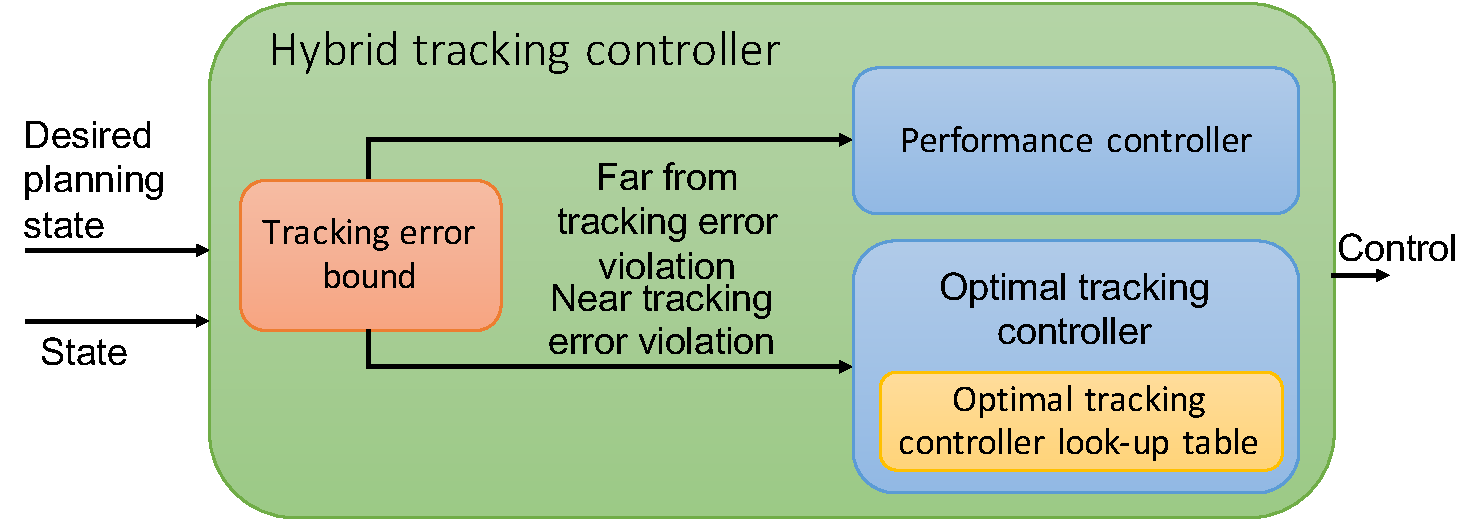
\includegraphics[width=0.9\columnwidth]{fig/hybrid_controller}
	\caption{Hybrid controller}
	\label{fig:hybrid_ctrl}
	\vspace{-.1in}
\end{figure}

To determine both the tracking error bound and safety controller functions/look-up tables, an offline framework is used as shown in Fig. \ref{fig:fw_offline}. The planning and tracking system dynamics are plugged into an HJ reachability computation, which computes a value function that acts as the tracking error bound function/look-up table. The spatial gradients of the value function comprise the safety controller function/look-up table. These functions are independent of the online computations---they depend only on the \textit{relative} states and dynamics between the planning and tracking systems, not on the absolute states along the trajectory at execution time.
\begin{figure}[h!]
  \centering
	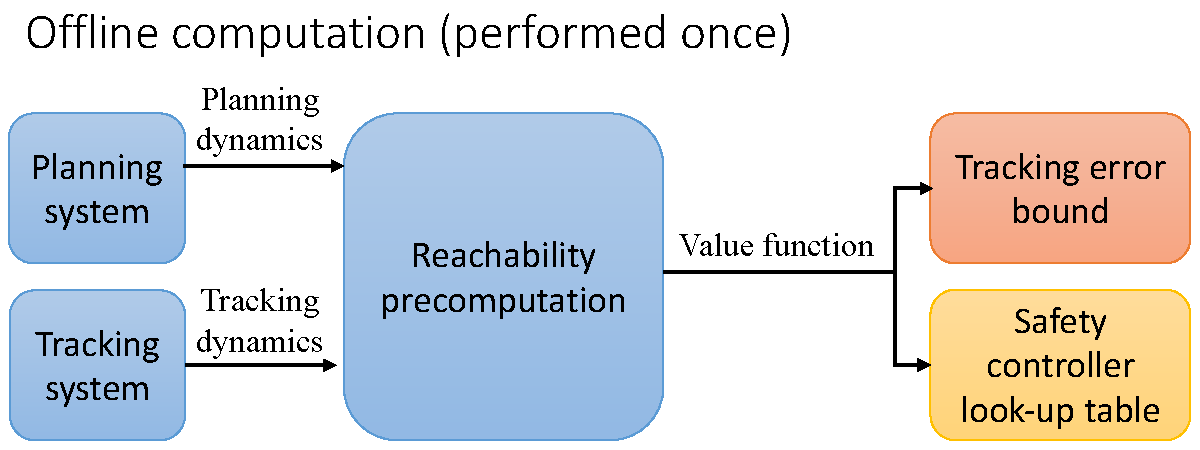
\includegraphics[width=0.9\columnwidth]{fig/framework_offline}
	\caption{Offline framework}
	\label{fig:fw_offline}
	%\vspace{-.1in}
\end{figure}
In the following sections we will first explain the precomputation steps taken in the offline framework. We will then walk through the online framework and provide a complete example.
%Besides the virtual state, the planner also takes into account any obstacles that must be avoided. In order to be robust to disturbances, planning must be done with a safety margin that accounts for disturbances. A safety margin that guarantees robustness despite the worst-case disturbance is given by a tracking error bound obtained in the offline HJ reachability computation, shown in Fig. \ref{fig:fw_offline} and explained in detail in \MCnote{Section \ref{}}. The virtual and real system dynamics are used to compute a value function, which simultaneously gives the tracking error bound and the safety controller look-up table used by the hybrid tracking controller.
%
%\textbf{Maybe put next paragraph in the introduction}
%
%There are many fast planners that could potentially do planning in real-time; however, these typically cannot account for disturbances in a provably safe way. In addition, complex system models with nonlinear dynamics complicate planning algorithms (non-convex for MPC, more difficult for RRT). On the other hand, HJ reachability is able to handle disturbances, and is agnostic to system dynamics. In addition, provably guarantees can be provided. However, HJ reachability and in general formal verification methods can be very expensive to compute.
%
%Refer to figure: planning level and safety level. 
%
%In the safety level, we start with the error dynamics, and we compute two things: bubble which is fed into planner to plan with extra margin, and error-feedback controller for real-time control. These two can be computed offline independent of the planned path.
%
%In the planning level, any planning method such as MPC, RRT, etc. (cite some things) can be used. The planning level does not need to take into account disturbances, and can use simple system dynamics or even no dynamics at all. In fact we will be using a simple RRT planner which simply provides paths, in the form of a sequence of line segments, which are not dynamically feasible. 
%framework of algorithm

% !TEX root = tracking.tex
\section{Offline Computations \label{sec:precomp}}

To precompute the tracking bound we set up a capture-avoid game between the real and virtual vehicles, which we then analyze using HJ reachability. In this game, the real system will try to "capture" the virtual system, while the virtual system is doing everything it can to avoid capture. By using reachability to analyze this game we will get a guaranteed bound on how far apart the two vehicles will ever be even when the virtual system is acting as inconveniently as possible. \MCnote{In addition, the tracking bound will be independent of the actual trajectory. (This is important to emphasize; Marco was confused about this.)}

\subsection{Relative Dynamics}
The states and dynamics of the real system, as defined in section \ref{sec:formulation}, are $\dot\tstate = \tdyn(\tstate, \tctrl, \dstb)$. The virtual system will have states $\pstate$, which we assume to be a subset of $\tstate$. The virtual system has dynamics $\dot\pstate = \pdyn(\pstate, \pctrl)$, with control $\pctrl$.
\SHnote{restrictions on $pctrl$?}

\textcolor{red}{introduce virtual dynamics, explain that it must be a subset of real system dynamics}
We now have the dynamics for the individual systems, but to set up the capture-avoid game we must first define the relative states and dynamics. We place the virtual vehicle at the origin by subtracting its states $(\pstate)$ from the real system's states $(\tstate)$. In this frame of reference $(\rstate)$ we are given the states of the real system relative to the virtual system. 

Dynamics of system
\begin{equation}
\dot\pstate = \pdyn(\pstate, \pctrl, \dstb)
\end{equation}

Dynamics of trajectory

\begin{equation}
\begin{aligned}
\rstate = \tstate - \ptmat\pstate\\
\dot\rstate = \rdyn(\rstate, \tctrl, \pctrl, \dstb)
\end{aligned}
\end{equation}

Matrix $\ptmat$ matches the common states of $\tstate$ and $\pstate$. The states $\rstate$ now represent the real state relative to the virtual state.

\subsection{Formalizing the Capture-Avoid Game}
Now that we have the relative dynamics between the two systems we must define a metric for the tracking error bound between these systems. We do this by defining an implicit surface function as a cost function $\errfunc(\rstate)$ in the new frame of reference \SHnote{requirements on $l(\rstate)$} Because the metric we care about is distance to the origin, this cost function can be as simple as negative distance in position space to the origin. An example can be seen in Figure \ref{fig:quad4D_example}-a, where the rings represent varying level sets of the cost function. The true vehicle will try to maximize this reward to reduce the relative distance, while the virtual vehicle will do the opposite.

\begin{figure}
	\centering
	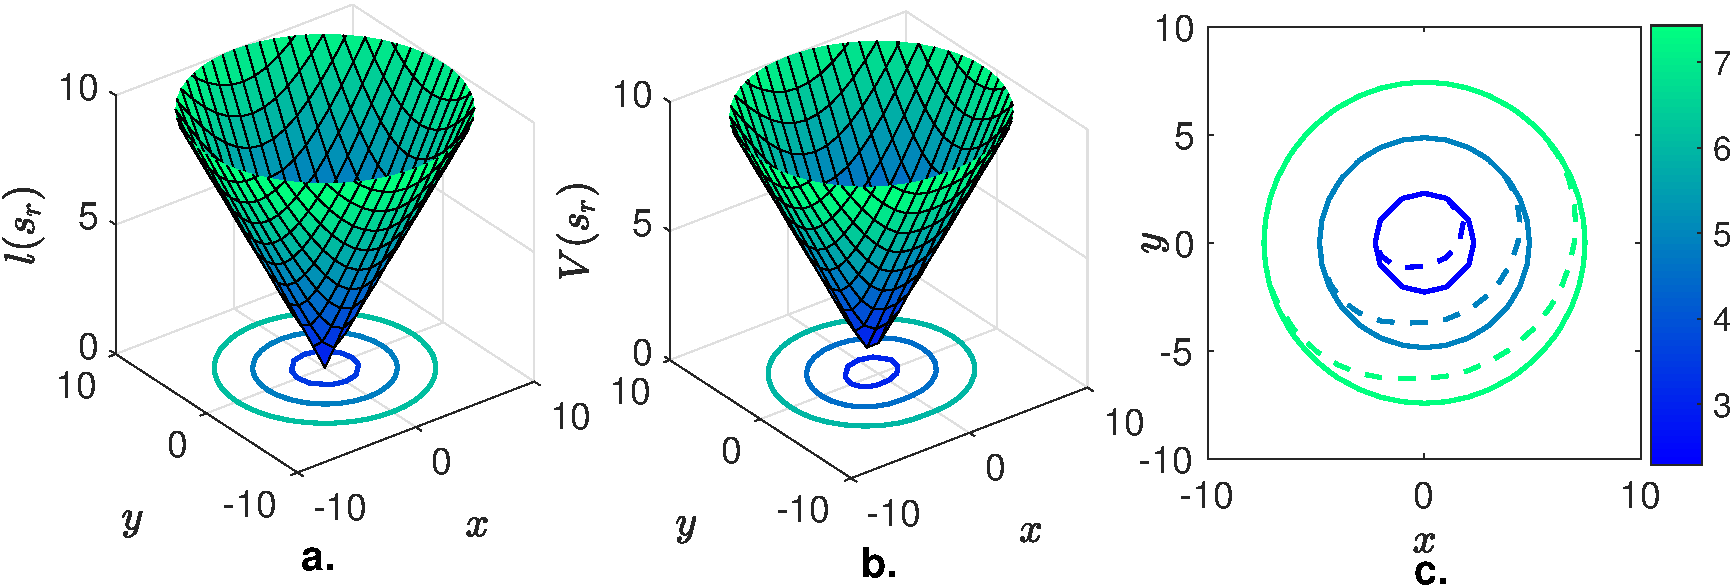
\includegraphics[width=0.5\textwidth]{fig/quad4D_example}
	\caption{\textcolor{red}{a) cost function, b) value function, c) level sets of both mapping initial state to tracking error bound}}
	\label{fig:quad4D_example}
\end{figure} 
 
 We want to find the farthest distance (and thus highest cost) that this game will ever reach when both players are acting optimally. Therefore we want to find a mapping between the initial state of the system and the maximum cost achieved over the time horizon. This mapping is through our value function, defined as: \MCnote{Time horizon, time variable notation, control/disturbance functions, trajectory notation}
 \begin{equation}
 \begin{aligned}
 	V(\rstate)= \sup_{\pctrl(\cdot)} \inf_{\tctrl(\cdot), \dstb(\cdot)} \big\{\sup_{\tvar\in [0, \thor]} \errfunc(\rtraj(\tvar; \rstate, 0, \pctrl(\cdot), \tctrl(\cdot)))\big\}
 	\end{aligned}
 \end{equation} 
 
 This is a modified version of the Hamilton-Jacobi formulation as described by \textcolor{red}{cite jaime, time varying reachability}. By implementing reachability analysis we solve for this value function over the time horizon. If the control authority of the real system is powerful enough to always eventually reach the virtual system, this value function will converge to an invariant solution for all time.  An example of this value function is in Figure \ref{fig:quad4D_example}-b. In the next section we will prove that the sub-level sets of this value function will map initial relative states to the guaranteed furthest possible tracking error over all time, as seen in Figure \ref{fig:quad4D_example}-c.
 
\subsection{Main Result}
 \begin{equation}
 \begin{aligned}
& \valfunc(\rstate, \thor) = \inf_{\pctrl(\cdot)} \sup_{\pctrl(\cdot), \dstb(\cdot)} \big\{\\
&\quad \max_{\tvar \in [0, \thor]} \errfunc(\rtraj(\tvar; \rstate, 0, \pctrl(\cdot), \pctrl(\cdot), \dstb(\cdot)))\big\} \\
& \valfunc(\rstate, \thor) = \max_{\tvar \in [0, \thor]} \errfunc(\rtraj^*(\tvar; \rstate, 0)) 
 \end{aligned}
  \end{equation}
 
 \begin{claim}
   \label{thm:main}
   Let $\thor_c \ge 0$, and suppose
   
   \begin{equation}
   \label{eq:conv_valfunc}
   \valfunc_\infty(\rstate) := \valfunc(\rstate, \thor) = \valfunc(\rstate, \thor_c) ~ \forall \thor \ge \thor_c.
   \end{equation}
   
   Then $\forall \tvar_1, \tvar_2$ with $\tvar_2 \ge \tvar_1$,
   
   \begin{equation}
   \label{eq:invariant}
   \valfunc_\infty(\rstate) \ge \valfunc_\infty\Big(\rtraj^*(\tvar_2;, \rstate, \tvar_1)\Big)
   \end{equation}
   
   \noindent where
   \begin{equation}
   \begin{aligned}
   & \rtraj^*(0;, \rstate, \tvar) := \rtraj(0; \rstate, \tvar, \pctrl^*(\cdot), \pctrl^*(\cdot), \dstb^*(\cdot))) \\
   & \pctrl^*(\cdot) = \arg \inf_{\pctrl(\cdot)} \sup_{\pctrl(\cdot), \dstb(\cdot)}\big\{ \\
   & \qquad \max_{\tvar \in [0, \thor]} \errfunc(\rtraj(0; \rstate, \tvar, \pctrl(\cdot), \pctrl(\cdot), \dstb(\cdot))) \big\}\\
   & \pctrl^*(\cdot) = \arg \sup_{\pctrl(\cdot)} \sup_{\dstb(\cdot)} \big\{ \\
   & \qquad \max_{t \in [0, \thor]} \errfunc(\rtraj(0; \rstate, \tvar, \pctrl(\cdot), \pctrl(\cdot), \dstb(\cdot))) \big\} \\
   & \dstb^*(\cdot) = \arg \sup_{\dstb(\cdot)} \big\{\max_{\tvar \in [0, \thor]} \errfunc(\rtraj(0; \rstate, \tvar, \pctrl(\cdot), \pctrl(\cdot),  \dstb(\cdot))) \big\}
   \end{aligned}
   \end{equation}
   
 \end{claim}
 
\textit{Proof:}

Assume $\thor \ge \thor_c$.

\begin{equation}
\begin{aligned}
\valfunc(\rstate, \thor) &= \valfunc_\infty(\rstate) = \max_{\tvar \in [0, \thor]} \errfunc(\rtraj^*(\tvar; \rstate, 0))\\
\end{aligned}
\end{equation}

By time-invariance
 \begin{equation}
 \begin{aligned}
 \valfunc_\infty(\rstate) &= \max_{\tvar \in [0, \thor]} \errfunc(\rtraj^*(\tvar; \rstate, 0)) \\
 &= \max_{\tvar \in [\thor_c-\thor, \thor_c]} \errfunc(\rtraj^*(\tvar; \rstate, \thor_c-\thor)) \\
 \end{aligned}
 \end{equation}  
 
Consider time subinterval:
 
 \begin{equation}
\begin{aligned}
\valfunc_\infty(\rstate) &= \max_{\tvar \in [0, \thor]} \errfunc(\rtraj^*(\tvar; \rstate, 0)) \\
&\ge \max_{\tvar \in [0, \thor_c]} \errfunc(\rtraj^*(\tvar; \rstate, \thor_c-\thor)) \\
\end{aligned}
\end{equation}  

Now look at trajectory $\rtraj^*(\tvar; \rstate, \thor_c-\thor)$:

\begin{equation}
\begin{aligned}
\rtraj^*(\tvar; \rstate, \thor_c-\thor) = \rtraj^*(\tvar; \rtraj^*(0; \rstate, \thor_c-\thor), 0)
\end{aligned}
\end{equation}

Continuing from value function:

\begin{equation}
\begin{aligned}
\valfunc_\infty(\rstate) &\ge \max_{\tvar \in [0, \thor_c]} \errfunc(\rtraj^*(\tvar; \rtraj^*(0; \rstate, \thor_c-\thor), 0)) \\
&= \valfunc_\infty(\rtraj^*(0; \rstate, \thor_c-\thor))
\end{aligned}
\end{equation} 
 
 By time-invariance again,
 
 \begin{equation}
 \begin{aligned}
 \valfunc_\infty(\rstate) &\ge \valfunc_\infty(\rtraj^*(\thor-\thor_c; \rstate, 0)) ~ \forall \thor\ge\thor_c \\
 \Leftrightarrow  \valfunc_\infty(\rstate) &\ge \valfunc_\infty(\rtraj^*(\tvar_2; \rstate, 0)) ~ \forall \tvar_2 \ge 0
 \end{aligned}
 \end{equation} 
 
   Since the system dynamics are time-invariant, we can pick $\tvar_2 = -\thor_c$ without loss of generality, and $\tvar_1 = -\thor$ to obtain the desired result. \hfill $\blacksquare$
 
\begin{rem}
  The interpretation of Theorem \ref{thm:main}, particularly \eqref{eq:invariant}, is that every level set of $\valfunc_\infty(\rstate)$ is invariant under the following conditions:
  \begin{itemize}
    \item The real system applies the optimal control which tries to track the virtual system;
    \item The virtual system applies the optimal virtual control that tries to escape from the real system;
    \item The real system experiences the worst-case disturbance.
  \end{itemize}
  
  In particular, the value of $\underline\valfunc := \valfunc_\infty(\rstate)$ can be interpreted as the smallest possible tracking error \MCnote{(we need to explicitly define tracking error)} given the above assumptions. The tracking error bound in Fig. \ref{fig:fw_online}, \ref{fig:hybrid_ctrl}, \ref{fig:fw_offline} is given by\footnote{In practice, since $\valfunc_\infty$ is obtained numerically, we set $\TEB = \{\rstate: \valfunc_\infty(\rstate) \le \underline\valfunc + \epsilon\}$ for some suitably small $\epsilon>0$} the set $\TEB = \{\rstate: \valfunc_\infty(\rstate) \le \underline\valfunc\}$.
  
  \MCnote{what if disturbances are not optimal?}
\end{rem}
 
 
 \begin{rem} 
   Theorem \ref{thm:main} is very similar to well-known results in differential game theory with a slightly different cost function \cite{}, and has been utilized in the context of using the subzero level set of $\valfunc_\infty$ as a backward reachable set for tasks such as collision avoidance or reach-avoid games \cite{}. In our work we do not assign special meaning to any particular level set, and instead consider all level sets at the same time. This effectively allows us to perform solve many simultaneous reachability problems in a single computation, thereby removing the need to check whether resulting invariant sets are empty, as was previously done in \MCnote{SPP paper \cite{}}.
 \end{rem}

\SHnote{say that this implicitly encodes all BRSs of initial states from which the tracking error reaches each level curve of the implicit value function}

% Computing capture basin (~2.5p)
%% HJ Reachability (~1p)
%% Relative dynamics, setup, etc. (~1p)
%% Capture basin computation (~0.5p)

% !TEX root = tracking.tex
\section{Online Computation \label{sec:online}}
Algorithm \ref{alg:algOnline} describes the online computation. The inputs are the tracking error function $\valfunc_\infty(\rstate)$ and the safety control function $\deriv_\infty(\rstate)$. 
Note that when discretized on a computer these functions will be look-up tables.

Lines \ref{ln:Istart}-\ref{ln:Iend} initialize the computation by setting the planning and tracking model states (and therefore the relative state) to zero. The tracking error bound in the planning frame of reference is computed using (\ref{eq:TEBp}). Note that by initializing the relative state to be zero we can use the smallest possible invariant $\TEB_\pstate$ for the entire online computation. 
\begin{algorithm}	
	\caption{Online Trajectory Planning}
	\label{alg:algOnline}
	\begin{algorithmic}[1]
		%\STATE Inputs: tracking error function $\valfunc(\rstate)$, safety control function $\deriv(\rstate)$
		\STATE \textbf{Initialization}: \label{ln:Istart}
 		\STATE $\TEB_\pstate(0) = \{\pstate: \valfunc_\infty(\rstate) \le \underline\valfunc\}$ \label{ln:Iend}
		\STATE Choose $\pstate, \tstate$ such that $\rstate \in $

		
		\WHILE{planning goal is not reached}
		\STATE \textbf{Tracking Error Bound Block}: \label{ln:obsStart}
		\STATE $\obsAug \leftarrow \obsSense + \TEB_\pstate(0)$ \label{ln:obsEnd}
		
		\STATE \textbf{Path Planner Block}:\label{ln:plannerStart}
		\STATE $\pstate_{next} \leftarrow \plannerfunc(\pstate, \obsAug)$\label{ln:plannerEnd}
		
		\STATE \textbf{Hybrid Tracking Controller Block}:\label{ln:controllerStart}
		\STATE $\rstate_{next} = \tstate - \ptmat\pstate_{next}$
		
		\IF{$\rstate_{next}$ is on boundary $\TEB_\pstate(0)$} 
		\STATE {use safety controller: $\tctrl \leftarrow \tctrl^*$ in \eqref{eq:opt_ctrl}}
		\ELSE \STATE{use performance controller: } 
          \STATE{$\tctrl \leftarrow$ desired controller} \ENDIF \label{ln:controllerEnd}
		
		\STATE \textbf{Tracking Model Block}: \label{ln:trackingStart}
		\STATE apply control $\tctrl$ to vehicle for a time step of $\dt$, save next state as $\tstate_{next}$ \label{ln:trackingEnd}
		
		\STATE \textbf{Planning Model Block}:\label{ln:planningStart}
		\STATE $\pstate = \tpmat\tstate_{next}$
		\STATE check if $\pstate$ is at planning goal
		\STATE reset states $\tstate = \tstate_{next}, \rstate = 0$ \label{ln:planningEnd}
		\ENDWHILE
	\end{algorithmic}
\end{algorithm}
The tracking error bound block is shown on lines \ref{ln:obsStart}-\ref{ln:obsEnd}. The sensor detects obstacles $\obsSense$ within the sensing distance around the vehicle. The sensed obstacles are augmented by $\TEB_\pstate(0)$ using the Minkowski sum. This is done to ensure that no unsafe path can be generated\footnote{The minimum allowable sensing distance is $\senseDist = 2\TEB_\pstate(0) + \dx$, where $\dx$ is the largest step in space that the planner can make in one time step.}.

%\SHnote{The planning distance is the distance that the path planner (and thus the planning model) may take for each iteration of the online algorithm, and is chosen to be $0< \dx \leq \TEB$. This in turn determines the time step of each iteration (as shown on line \ref{ln:dt}): , where $v_{max}$ is the maximum speed of the planning model.}

 The path planner block (lines \ref{ln:plannerStart}-\ref{ln:plannerEnd}) takes in the planning model state $\pstate$ and the augmented obstacles $\obsAug$, and outputs the next state of the planning system $\pstate_{next}$. The hybrid tracking controller block (lines \ref{ln:controllerStart}-\ref{ln:controllerEnd}) first computes the updated relative state $\rstate_{next}$. If the $\rstate_{next}$ is on the tracking bound $\TEB_\pstate(0)$, the safety controller must be used to remain within the safe bound. The safety control is given by:
\begin{equation}
  \label{eq:opt_ctrl}
	\tctrl^* = \arg\min_{\tctrl\in\tcset} \max_{\pctrl\in\pcset, \dstb\in\dset} \nabla\valfunc(\rstate_{next}) \cdot \rdyn(\rstate_{next},\tctrl,\pctrl,\dstb)
\end{equation}
For many practical systems (such as control affine systems), this minimization can be found extremely quickly.

If the relative state is not on the tracking boundary, a performance controller may be used. For the example in Section \ref{sec:results} the safety and performance controllers are identical, but in general this performance controller can suit the needs of the individual applications.

The control $\tctrl^*$ is then applied to the physical system in the tracking block (lines \ref{ln:trackingStart}-\ref{ln:trackingEnd}) for a time period of $\dt$. The next state is saved as $\tstate_{next}$. This then updates the planning model state in the planning model block (lines \ref{ln:planningStart}-\ref{ln:planningEnd}). We repeat this process until the planning goal has been reached.
% online part of framework

% !TEX root = tracking.tex
\section{Numerical examples}

\subsection{5D-3D example with FSM planner \label{sec:reach_planner}}

\subsubsection{Offline computation}
\subsubsection{Online sensing and planning with FSM }


% !TEX root = tracking.tex
\subsection{10D quadrotor-3D single integrator example with RRT\label{sec:resultsRRT}}

Our second example involves a 10D near-hover quadrotor developed in \cite{Bouffard12} as the tracking model and a single integrator in 3D space as planning model.
Planning is done using RRT, a well-known sampling-based planner that quickly produces geometric paths from a starting position to a goal position \cite{Kuffner2000,Kavraki1996}.
Paths given by the RRT planner is converted to time-stamped trajectories by placing a maximum velocity in each dimension along the generated geometric paths.

The dynamics of tracking model and of the 3D single integrator is as follows:

\begin{equation}
\label{eq:Quad10D_dyn}
\begin{bmatrix}
\dot{x}\\
\dot{v_x}\\
\dot{\theta_x}\\
\dot\omega_x\\
\dot{y}\\
\dot{v_y}\\
\dot{\theta_y}\\
\dot\omega_y\\
\dot{z}\\
\dot{v_z}
\end{bmatrix}
=
\begin{bmatrix}
v_x + d_x\\
g \tan \theta_x\\
-d_1 \theta_x + \omega_x\\
-d_0 \theta_x + n_0 a_x\\
v_y + d_y\\
g \tan \theta_y\\
-d_1 \theta_y + \omega_y\\
-d_0 \theta_y + n_0 a_y\\
v_z + d_z\\
k_T a_z - g
\end{bmatrix}, \quad
\begin{bmatrix}
\dot{\hat x}\\
\dot{\hat y}\\
\dot{\hat z}\\
\end{bmatrix} =
\begin{bmatrix}
\hat v_x \\
\hat v_y \\
\hat v_z
\end{bmatrix},
\end{equation}
\noindent where quadrotor states $(x, y, z)$ denote the position, $(v_x, v_y, v_z)$ denote the velocity, $(\theta_x, \theta_y)$ denote the pitch and roll, and $(\omega_x, \omega_y)$ denote the pitch and roll rates. 
The controls of the 10D system are $(u_x, u_y, u_z)$, where $u_x$ and $u_y$ represent the desired pitch and roll angle, and $u_z$ represents the vertical thrust.

The 3D system controls are $(\hat v_x, \hat v_y, \hat v_z)$, and represent the velocity in each positional dimension. 
The disturbances in the 10D system $(\dstb_x, \dstb_y, \dstb_z)$ are caused by wind, which acts on the velocity in each dimension. 

The model parameters are chosen to be $d_0=10$, $d_1=8$, $n_0=10$, $k_T=0.91$, $g=9.81$, $|u_x| |u_y| \le \pi/9$, $u_z \in [0, 1.5g]$, $|\hat v_x|, |\hat v_y|, |\hat v_z| \le 0.5$.
The disturbance bounds were chosen to be $|d_x|, |d_y|, |d_z| \le 0.1$.

\subsubsection{Offline computation}
We define the relative system states to consist of the error states, or relative position $(x_r, y_r, z_r)$, concatenated with the rest of the state variables of the 10D quadrotor model.
Defining $\rtrans = \mathbf I_{10}$ and 

\begin{equation*}
\ptmat = 
\begin{bmatrix}
  \begin{bmatrix} 1 \\ \mathbf 0_{3 \times 1} \end{bmatrix} 
    & \mathbf 0_{4\times 1} 
    & \mathbf 0_{4\times 1} \\
  \mathbf 0_{4\times 1} 
    & \begin{bmatrix} 1 \\ \mathbf 0_{3 \times 1} \end{bmatrix} 
    &  \mathbf 0_{4\times 1} \\
  \mathbf 0_{2\times 1} 
    & \mathbf 0_{2\times 1} 
    & \begin{bmatrix} 1 \\ 0 \end{bmatrix}
\end{bmatrix},
\end{equation*}

\noindent we obtain the following relative system dynamics:

\begin{equation}
\label{eq:Quad10DRel_dyn}
\begin{bmatrix}
\dot x_r\\
\dot v_x\\
\dot \theta_x\\
\dot\omega_x\\
\dot y_r\\
\dot v_y\\
\dot \theta_y\\
\dot\omega_y\\
\dot z_r\\
\dot v_z
\end{bmatrix} =
\begin{bmatrix}
v_x - \hat v_x + d_x\\
g \tan \theta_x\\
-d_1 \theta_x + \omega_x\\
-d_0 \theta_x + n_0 u_x\\
v_y - \hat v_y + d_y\\
g \tan \theta_y\\
-d_1 \theta_y + \omega_y\\
-d_0 \theta_y + n_0 u_y\\
v_z - \hat v_z + d_z\\
k_T u_z - g
\end{bmatrix}.
\end{equation}


The relative system dynamics given in \eqref{eq:Quad10DRel_dyn} is decomposable into three independent subsystems involving the sets of variables $(x_r, v_x, \theta_x, \omega_x)$, $(x_y, v_y, \theta_y, \omega_y)$, $(z_r, v_z)$, allowing us to choose the error function to be also in the decomposable form of $\errfunc(\rstate) = \max(x_r^2, y_r^2, z_r^2)$, so that we can solve \eqref{eq:HJVI} tractably since each subsystem is at most 4D \cite{Chen2016DecouplingJournal}. 

The left subplot of Fig. \ref{fig:valfuncRRT} shows the the projection of the value function $\valfunc$ onto the $(x_r, v_x)$ space resulting from solving \eqref{eq:HJVI} over an increasingly long time horizon.
Starting from $\tau=0$, we have that $\errfunc(\rstate) = \valfunc(\rstate, 0)$.
As $\tau$ increases, the value function evolves according to \eqref{eq:HJVI}, and eventually converges when $\tau$ reaches $3.5$.
This implies that $\valfunc_\infty(\rstate) = \valfunc(\rstate, \tau=3.5)$, since we would still obtain the same function even if we let $\tau$ approach infinity.
The horizontal plane shows the minimum value, $\underline\valfunc = 0.3$, which corresponds to a TEB of approximately 0.55.

The right subplot of Fig. \ref{fig:valfuncRRT} shows the $\underline\valfunc = 0.3$ level set of value function projection, which is the projection, onto the $(x_r, v_x)$ space, of the TEB $\TEB_{\estate, \infty}$ according to \eqref{eq:TEBp:inf}.
The range of $x_r$ provides the TEB used for the planner, $\TEB_{\pstate, \infty}$, as given in \eqref{eq:TEBp:inf}.

The value function and TEB in the $(y_r, v_y, \theta_y, \omega_y)$ and $(z_r, v_z)$ spaces are combined together to form the TEB in 3D positional space.
For conciseness, these value functions are not shown; however, one can see the resulting TEB in Fig. \ref{fig:simRRT} and \ref{fig:simRRT_combined} as the translucent red box.

Offline computations were done on a laptop with an Intel Core i7 4702HQ CPU using a MATLAB implementation of level set methods \cite{Mitchell07c} used for solving \eqref{eq:HJVI}.
The 4D computations were done on a $61\times 61 \times 41 \times 41$ grid, took approximately 12 hours, and required approximately 300 MB of RAM.
The 2D computation in the $(z_r, v_z)$ space was done on a $101 \times 101$ grid, took approximately 15 seconds, and required negligible RAM.

\begin{figure}
  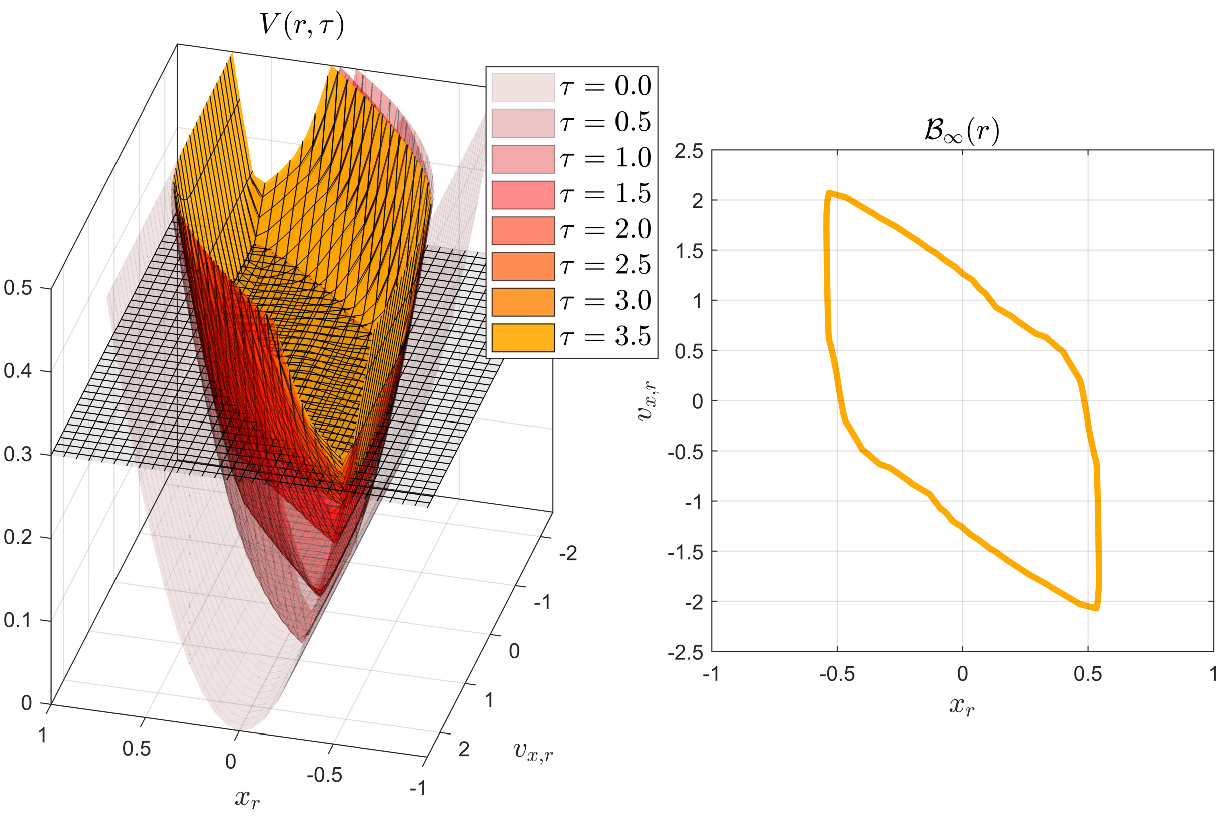
\includegraphics[width=\columnwidth]{fig/Q10D_Q3D/valfunc}
  \caption{}
  \label{fig:valfuncRRT}
\end{figure}

\subsubsection{Online sensing and planning}
The simulation involving the 10D quadrotor model tracking the 3D single integrator is shown in Fig. \ref{fig:simRRT} and \ref{fig:simRRT_combined}.
Here, the system aims to start at $(x,y,z) = (-12, 0, 0)$ and reach $(12, 0, 0)$. 
Three rectangular obstacles, which make up the constraints $\constr$, are present and initially unknown.
Before the obstacles are sensed by the system, they are shown in gray, and when the tracking system is within 1.5 units away from a part of an obstacle, that part is revealed to the system as the sensed obstacles which form the sensed constraints $\constrSense$.
The sensed obstacles are colored red.
Whenever new obstacles are revealed, the planning system replans using RRT, in real time, a trajectory to the goal while avoiding the augmented constraint set $\constrAug$.

Fig. \ref{fig:simRRT} shows the entire trajectory, with the end of the trajectory being close to the goal position.
The planning system state is shown as a small green star, and the translucent box around it depicts the TEB: the tracking system position is guaranteed to reside within this box.
Therefore, as long as the planning system plans in a way such that the the TEB does not intersect with the obstacles, the tracking system is guaranteed to be safe.
Due to the random nature of RRT, during the simulation the system appears to randomly explore to look for an unobstructed path to the obstacle; we did not implement any exploration algorithms.

Fig. \ref{fig:simRRT_combined} shows three different time snapshots of the simulation.
At $t=8$, the planning system has sensed a portion of the previously unknown obstacles, and replans, so that the path deviates from a straight line from the initial position to the goal position.
The subplot showing $t = 47.7$ is rotated to show the trajectory up to this time from a more informative view angle.
Here, the tracking system has safely passed by the first planar obstacle, and is moving around the second. 
Note that the TEB never intersects the obstacles, implying that the tracking system is guaranteed to avoid collision with the obstacles, since it is guaranteed to stay within the TEB.
At $t=83.5$, the tracking system safely passes by the last planar obstacle.

\begin{figure}
  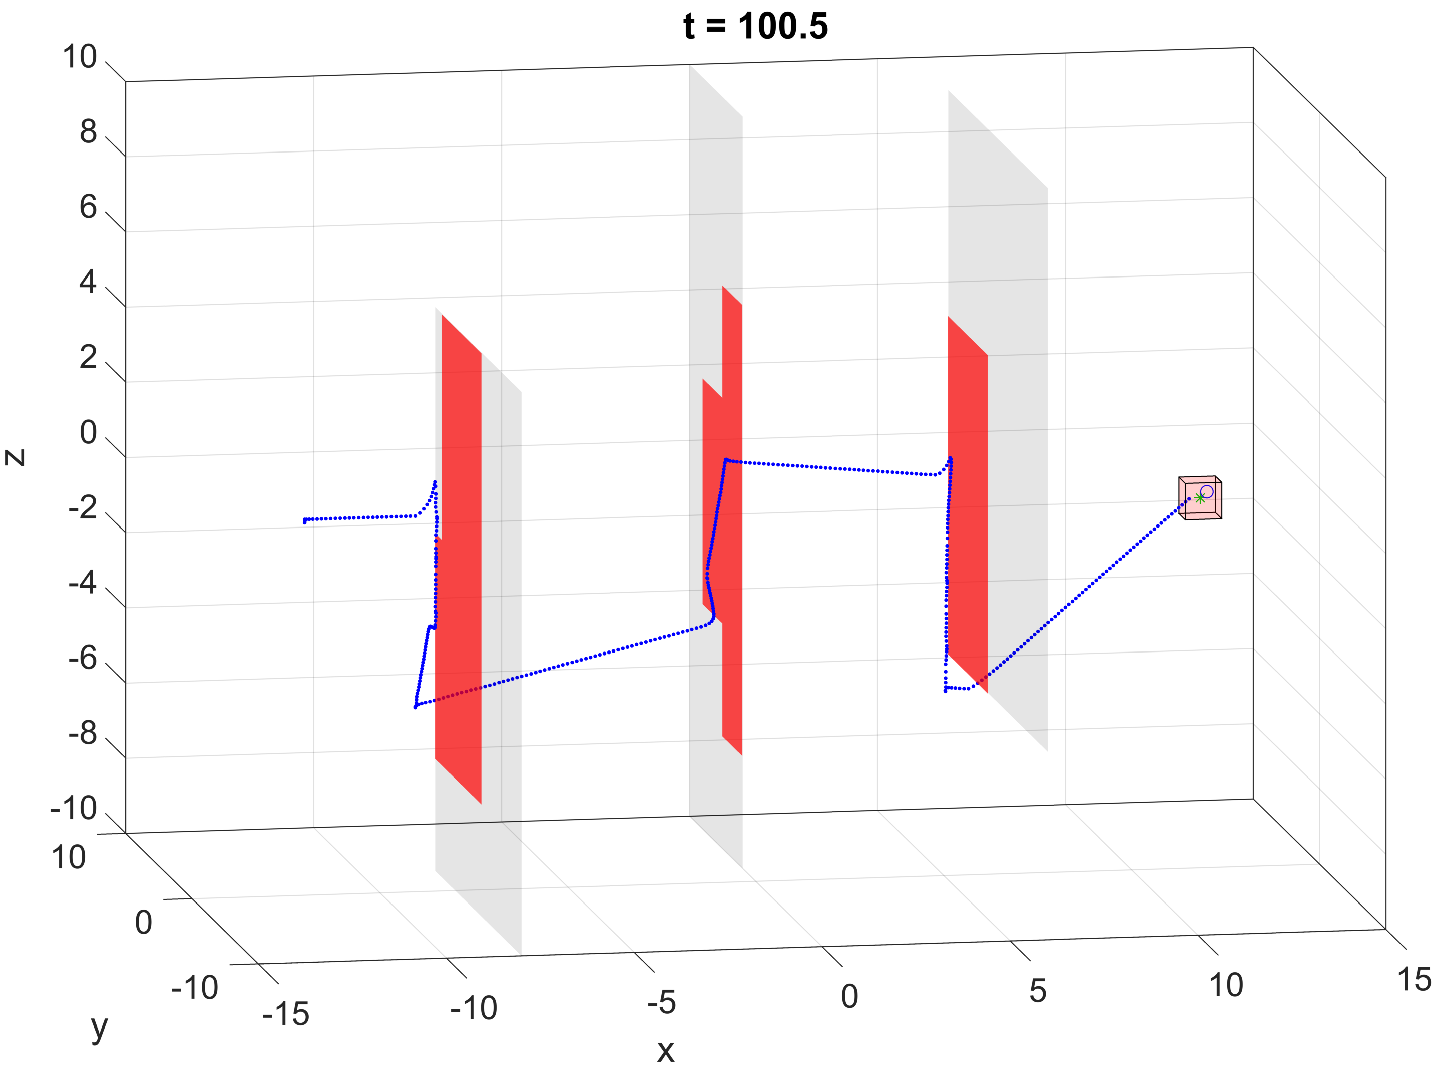
\includegraphics[width=\columnwidth]{fig/Q10D_Q3D/10050}
  \caption{Simulation of the 10D quadrotor tracking (trajectory shown in blue) a 3D single integrator (position shown as green star inside red box) in order to perform real-time robust planning. The system senses initially unknown obstacles (gray), which are revealed (revealed parts shown in red) as the system approaches them. Replanning is done in real-time by RRT when new obstacles are sensed. The TEB is shown as the red box, and is the set of positions that the 10D quadrotor is guaranteed to remain within.}
  \label{fig:simRRT}
\end{figure}

\begin{figure}
  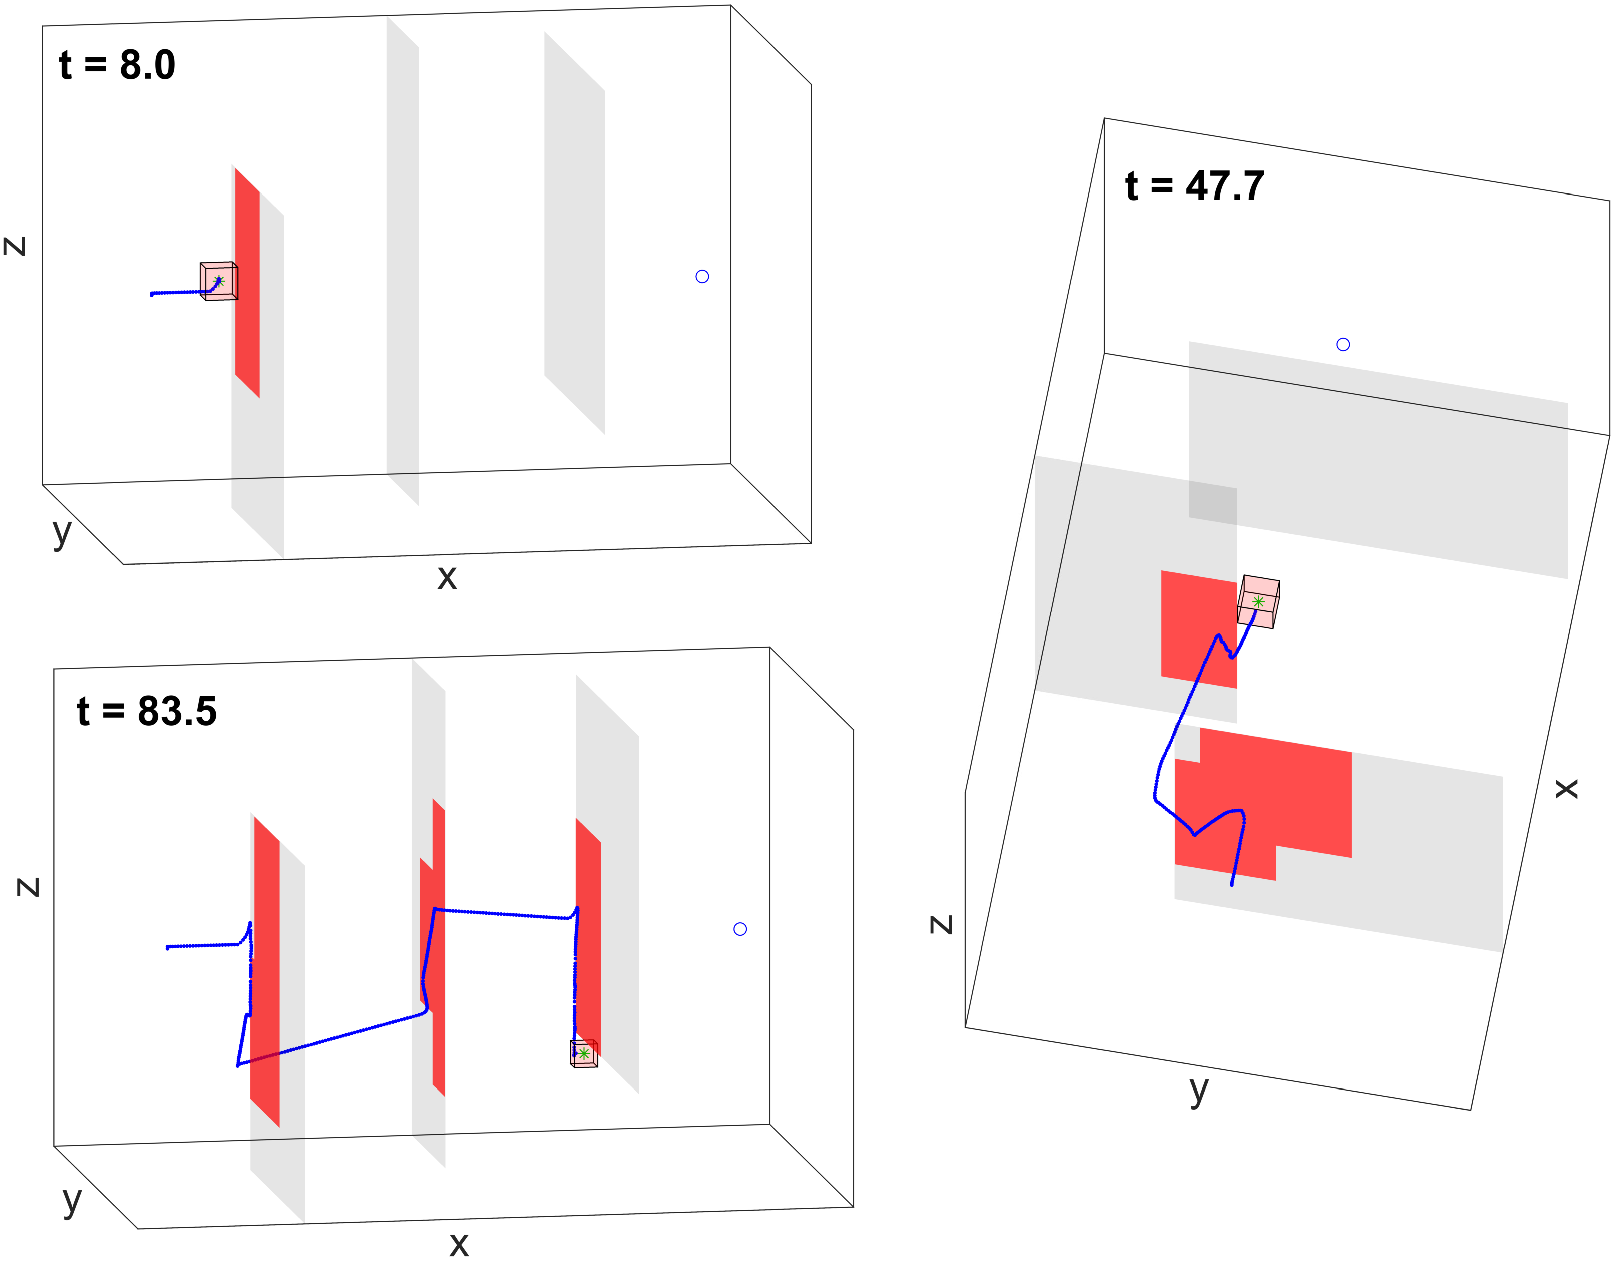
\includegraphics[width=\columnwidth]{fig/Q10D_Q3D/combined}
  \caption{Three time snapshots of the simulation in Fig. \ref{fig:simRRT}.}
  \label{fig:simRRT_combined}  
\end{figure}

Fig. \ref{fig:tracking_error_RRT} shows the maximum tracking error, in the three positional dimensions over time.
The red points indicate the time points at which the optimal tracking controller from Eq. \eqref{eq:opt_ctrl_inf} was used; this is the safety controller depicted in Fig. \ref{fig:hybrid_ctrl}. 
The blue points indicate the time points at which a performance controller, also depicted in Fig. \ref{fig:hybrid_ctrl}, was used.
For the performance controller, we used a simple proportional controller that depends on the tracking error in each positional dimension; this controller is used whenever the tracking error is less than a quarter of the TEB.
From Fig. \ref{fig:tracking_error_RRT}, one can observe that the tracking error is always less than the TEB implied by the value function.
The disturbance was chosen to be uniformly random within the chosen bounds.


\begin{figure}
  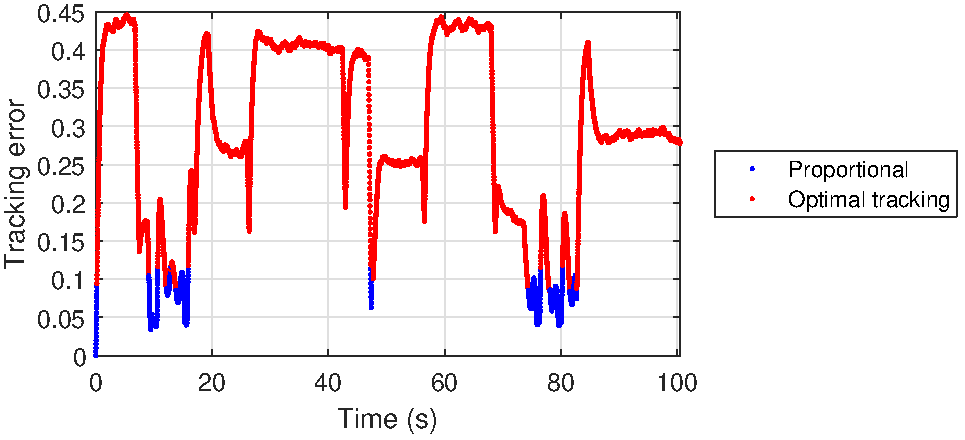
\includegraphics[width=\columnwidth]{fig/Q10D_Q3D/tracking_error}
  \caption{Tracking error over time for the 10D-3D example. The red dots indicate that the optimal tracking controller in \eqref{eq:opt_ctrl_inf} is used, while the blue dots indicate that an LQR controller for the linearized system is used. The tracking error stays well below the predicted TEB of 0.55.}
  \label{fig:tracking_error_RRT}  
\end{figure}

The simulation was done in MATLAB on a desktop computer with an Intel Core i7 2600K CPU.
The time was discretized in increments of 0.01.
Per iteration, planning with RRT using a simple multi-tree RRT planner implemented in MATLAB modified from \cite{Gavin2013} took on average 5 ms, and computing the tracking controller took on average 5.5 ms. 



% !TEX root = tracking.tex
\subsection{8D quadrotor-4D double integrator example with MPC \label{sec:resultsMPC}}

In this section, we demonstrate the online computation framework in Algorithm \ref{alg:algOnline} with an 8D quadrotor example. 
Unlike in Sections \ref{sec:reach_planner} and \ref{sec:resultsRRT}, we consider a time-varying TEB and utilize MPC as the online planner.
In addition, the TEB depends on both position and speed, as opposed to just position.

First we define the 8D dynamics of the near-hover quadrotor, and the 4D dynamics of a double integrator, which serves as the planning system to be used in MPC:

\begin{equation}
\label{eq:Quad8D_dyn}
\begin{bmatrix}
\dot x\\
\dot v_x\\
\dot \theta_x\\
\dot \omega_x\\
\dot y\\
\dot v_y\\
\dot \theta_y\\
\dot \omega_y
\end{bmatrix} =
\begin{bmatrix}
v_{x,s} + d_x\\
g \tan \theta_x\\
-d_1 \theta_x + \omega_x\\
-d_0 \theta_x + n_0 a_x\\
v_y + d_y\\
g \tan \theta_y\\
-d_1 \theta_y + \omega_y\\
-d_0 \theta_y + n_0 a_y
\end{bmatrix}, \quad
\begin{bmatrix}
\dot {\hat x}\\
\dot {\hat v}_x\\
\dot {\hat y}\\
\dot {\hat v}_y\\
\end{bmatrix} =
\begin{bmatrix}
\hat v_x\\
\hat a_x\\
\hat v_y\\
\hat a_y\\
\end{bmatrix}
\end{equation}

\noindent where the states, controls, and disturbances are the same as the first 8 components of the dynamics in \eqref{eq:Quad10D_dyn}. 
The position $(\hat x,\hat y)$ and velocity $(\hat v_x, \hat v_y)$ are the states of the 4D system. 
The controls are $(\hat a_x, \hat a_y)$, which represent the acceleration in each positional dimension. 

The model parameters are chosen to be $d_0=10$, $d_1=8$, $n_0=10$, $k_T=0.91$, $g=9.81$, $|u_x|, |u_y| \le \pi/9$, $|\hat a_x|, |\hat a_y| \le 1$, $|\dstb_x|, |\dstb_y| \le 0.2$.

\subsubsection{Offline precomputation}
We define the relative states to be the error states $(x_r, v_{x,r}, y_r, v_{y,r})$, which are the relative position and velocity, concatenated with the rest of the states in the 8D system.
Defining $\rtrans = \mathbf I_8$ and 

\begin{equation*}
\ptmat = 
\begin{bmatrix}
  \begin{bmatrix}
    1 & \mathbf 0_{1 \times 3} \\
    \mathbf 0_{3 \times 1} & \mathbf 0_{3 \times 3}
  \end{bmatrix} & \mathbf 0_{4\times 4} \\
  \mathbf 0_{4\times 4} & \begin{bmatrix}
    1 & \mathbf 0_{1 \times 3} \\
    \mathbf 0_{3 \times 1} & \mathbf 0_{3 \times 3}
  \end{bmatrix} 
\end{bmatrix},
\end{equation*}

\noindent we obtain the following relative system dynamics:
\begin{equation}
\label{eq:Quad8DRel_dyn}
\begin{bmatrix}
\dot x_r\\
\dot v_{x,r}\\
\dot \theta_x\\
\dot \omega_x\\
\dot y_r\\
\dot v_{y,r}\\
\dot \theta_y\\
\dot \omega_y\\
\end{bmatrix} =
\begin{bmatrix}
v_{x,r} + \dstb_x\\
g \tan \theta_x - \hat a_x\\
-d_1 \theta_x + \omega_x\\
-d_0 \theta_x + n_0 a_x\\
v_{y,r} + \dstb_y\\
g \tan \theta_y - \hat a_y\\
-d_1 \theta_y + \omega_y\\
-d_0 \theta_y + n_0 a_y\\
\end{bmatrix}.
\end{equation}


As in the 10D-3D example in Section \ref{sec:resultsRRT}, the relative dynamics are decomposable into two 4D subsystems, and so computations were done in 4D space.
On a laptop computer with an Intel Core I7 4702HQ CPU, the offline computation on a $\times\times$ grid took approximately ... and  required approximately GB of RAM using a C++ implementation of level set methods for solving \eqref{eq:HJVI}.

\subsubsection{Online computation}
%
We utilize the MPC design introduced in \cite{Zhang2017} for the online path planning. See in Problem~\ref{pr: MPC}.
%
\begin{problem}\label{pr: MPC}
\begin{align*}
\min_{\mathbf{p},\mathbf{u}}  & \quad \sum^{N-1}_{k=0} l(p_k,u_k) + l_f(p_N-p_f)  \\
s.t. \quad & p_0 = p_{init},\\
&p_{k+1} = f_p(p_k,u_k),\\
& p_k \in \mathbb{P}_k ,\enspace u_k \in \mathbb{U},\\
& \mathbb{S}(p_k)\cap\constrAug(t_k) = \emptyset
\end{align*}
\end{problem}
where $l(\cdot,\cdot)$ and $l_f(\cdot)$ are convex stage and terminal cost functions, $N$ is the horizon for the MPC problem, and $t_k = t_0 + k \MCnote{\Delta t}$ denotes the current time used in simulation, with $t_0$ being the time when the MPC problem starts to be solved and $\Delta t$ the MPC sampling interval. The dynamical system $f_p(\cdot,\cdot)$ is set to be a discretized model of the 4D dynamics in \eqref{eq:Quad8D_dyn}. The state and input sequences along the horizon  are denoted by $\mathbf{p}=[p^{T}_0,p^{T}_1,\cdots,p^{T}_N]^{T}$ and $\mathbf{u}=[u^{T}_0,u^{T}_1,\cdots,u^{T}_{N-1}]^{T}$. The velocity states are subject to convex time-varying constraints:
%
\begin{equation}
(\hat v_{x,k},\hat v_{y,k}) \subset p_k \in \mathbb{P}_k :=\mathbb{P}\oplus\TEB_\pstate(t_k) \enspace ,
\end{equation}
%
where $\oplus$ denotes the Minkowski addition, $\mathbb{P}$ denotes the original state constraint, and $\TEB_\pstate(t_k)$ is the tracking error bound sampled at $t_k$, respectively. Given the state vector $p_k$, we denote the position of the controlled object by $(\hat x_k,\hat y_k) := \mathbb{S}(p_k)\subseteq \mathbb{R}^{2}$. To avoid collision with obstacles, $\mathbb{S}(p_k)$ is subject to the following constraint: 
%
\begin{equation}
\mathbb{S}(p_k)\cap\constrAug(t_k) = \emptyset \enspace ,
\end{equation}
%
with 
%
\begin{equation}
\constrAug(t_k) := \constrSense(t_0)\oplus\TEB_\pstate(t_k) \enspace .
\end{equation}
%
where $\constrSense(t_0)$ denotes the obstacles sensed at $t_0$.

In this paper, we represent the obstacles as polytopes, i.e., $\constrSense = \cap \constr^{i}$ with $\constr^{i}:= \{z\in\mathbb{R}^{n} \mid A^{i}z\leq b^{i}\}$ for $i = 1,\cdots ,M$. We follow the approach presented in \cite{Zhang2017} to compute a local minimal solution, by involving extra variables $\lambda^{i}$ for each obstacle $\constr^{i}$ and reformulating the collision avoidance constraint equivalently as follows: 
%
\begin{equation}
\exists \lambda^{i} >0, \; \mbox{s.t.} \; (A^{i} \mathbb{S}(p_k) - b^{i})^{T}\lambda^{i}  > 0, \; \|A^{i^{T}}\lambda^{i}\|_2\leq 1\enspace .
\end{equation}
%
Note that the collision avoidance constraint causes the MPC problem to be non-convex and thus computationally expensive.

The procedure of finding the next state of the planning system using the proposed MPC planner is summarized in Algorithm \ref{alg:mpc}.
%
\begin{algorithm}	
	\caption{MPC Path Planner Block}
	\label{alg:mpc}
	\begin{algorithmic}[1]
		\STATE \textbf{Initialization}:
 		\STATE Set initial time and states: $t_0 \leftarrow \tvar, \pstate_0 \leftarrow \pstate$
		\IF{MPC is ready to re-plan}
			\STATE Solve MPC for the optimal control sequence: $\mathbf{u}_t \leftarrow \text{Problem\ref{pr: MPC}} (t_0,p_0,\constrAug)$
		\ENDIF
        \STATE Get the current control: $u(t) \leftarrow u_k \in \mathbf{u}_t$ such that $t \in [t_0 + k \Delta t, t_0 + (k+1) \Delta t]$
		\STATE Output the next state: $\pstate_\text{next} = f_p(p,u(t))$
	\end{algorithmic}
\end{algorithm}

\subsubsection{Simulations}

%The values for parameters $d_0,d_1,n_0,k_T,g$ used for the 8D model are: $d_0=10,d_1=8,n_0=10,k_T=0.91,g=9.81$.

%The 8D control bounds are $|a_x|,|a_y|\leq10$ degrees.

%The 4D control bound is $\|(\hat a_x,\hat a_y)\|_2\leq1.0$ m/s$^{2}$.

%The disturbance bounds are $|d_{v_x}|,|d_{v_y}|\leq0.1$ m/s.

%The sensing range is $\MCnote{r = 5}$ meters.

For the MPC problem we used a horizon $N=8$ with sampling interval $\Delta t = 0.2$ s.

Implementation of the MPC planner was based on MATLAB and \texttt{ACADO Toolkit} \cite{Houska2011a}. The nonlinear MPC problem was solved using an online active set strategy implemented in \texttt{qpOASES} \cite{Ferreau2014}. All the simulation results were obtained on a laptop with Ubuntu 14.04 LTS operating system and a Core i5-4210U CPU. The MPC planner re-plans every 0.8 s with an average computational time of 0.37 s for each planning loop. The frequency of control was once every 0.1 s for the 8D quadrotor system.

\MCnote{Simulation figures and explanations to be added.}
% Numerical Simulations (1-2p)
%% demonstrate feasibility (~.5)
%% real-time computation load (~.5)
%% comparison to other methods (~.5)

% !TEX root = tracking.tex
\section{Conclusions and Future work}
In this paper we introduced our new tool FaSTrackHD: Fast and Safe Tracking for High Dimensional systems. This tool can be used to add robustness to various path and trajectory planners without sacrificing fast online computation. So far this tool can be applied to unknown environments with a limited sensing range and static obstacles. We are excited to explore several future directions for FaSTrackHD in the near future, including exploring robustness for moving obstacles, adaptable error bounds based on external disturbances, and demonstration on a variety of planners.
% Conclusion (0.5p)

%%%%%%%%%%%%%%%%%%%%%%%%%%%%%%%%%%%%%%%%%%%%%%%%%%%%%%%%%%%%%%%%%%%%%%%%%%%%%%%%
%\addtolength{\textheight}{1cm}   % This command serves to balance the column lengths
                                  % on the last page of the document manually. It shortens
                                  % the textheight of the last page by a suitable amount.
                                  % This command does not take effect until the next page
                                  % so it should come on the page before the last. Make
                                  % sure that you do not shorten the textheight too much.

\bibliographystyle{IEEEtran}
\bibliography{references}
\end{document}
